\documentclass[10pt]{beamer}\usepackage[]{graphicx}\usepackage[]{color}
% maxwidth is the original width if it is less than linewidth
% otherwise use linewidth (to make sure the graphics do not exceed the margin)
\makeatletter
\def\maxwidth{ %
  \ifdim\Gin@nat@width>\linewidth
    \linewidth
  \else
    \Gin@nat@width
  \fi
}
\makeatother

\definecolor{fgcolor}{rgb}{0.345, 0.345, 0.345}
\newcommand{\hlnum}[1]{\textcolor[rgb]{0.686,0.059,0.569}{#1}}%
\newcommand{\hlstr}[1]{\textcolor[rgb]{0.192,0.494,0.8}{#1}}%
\newcommand{\hlcom}[1]{\textcolor[rgb]{0.678,0.584,0.686}{\textit{#1}}}%
\newcommand{\hlopt}[1]{\textcolor[rgb]{0,0,0}{#1}}%
\newcommand{\hlstd}[1]{\textcolor[rgb]{0.345,0.345,0.345}{#1}}%
\newcommand{\hlkwa}[1]{\textcolor[rgb]{0.161,0.373,0.58}{\textbf{#1}}}%
\newcommand{\hlkwb}[1]{\textcolor[rgb]{0.69,0.353,0.396}{#1}}%
\newcommand{\hlkwc}[1]{\textcolor[rgb]{0.333,0.667,0.333}{#1}}%
\newcommand{\hlkwd}[1]{\textcolor[rgb]{0.737,0.353,0.396}{\textbf{#1}}}%
\let\hlipl\hlkwb

\usepackage{framed}
\makeatletter
\newenvironment{kframe}{%
 \def\at@end@of@kframe{}%
 \ifinner\ifhmode%
  \def\at@end@of@kframe{\end{minipage}}%
  \begin{minipage}{\columnwidth}%
 \fi\fi%
 \def\FrameCommand##1{\hskip\@totalleftmargin \hskip-\fboxsep
 \colorbox{shadecolor}{##1}\hskip-\fboxsep
     % There is no \\@totalrightmargin, so:
     \hskip-\linewidth \hskip-\@totalleftmargin \hskip\columnwidth}%
 \MakeFramed {\advance\hsize-\width
   \@totalleftmargin\z@ \linewidth\hsize
   \@setminipage}}%
 {\par\unskip\endMakeFramed%
 \at@end@of@kframe}
\makeatother

\definecolor{shadecolor}{rgb}{.97, .97, .97}
\definecolor{messagecolor}{rgb}{0, 0, 0}
\definecolor{warningcolor}{rgb}{1, 0, 1}
\definecolor{errorcolor}{rgb}{1, 0, 0}
\newenvironment{knitrout}{}{} % an empty environment to be redefined in TeX

\usepackage{alltt}


%\input{slides_header.tex}
\usepackage{graphicx}
\usepackage{hyperref, url}
\hypersetup{colorlinks,citecolor=myorange,filecolor=red,linkcolor=brown,urlcolor=blue}

\usepackage{longtable,booktabs}
\usepackage{amssymb,amsmath}
\usepackage{animate}
\usepackage{subfig}
\usepackage{tikz}
\usetikzlibrary{shapes.geometric, arrows,shapes.symbols,decorations.pathreplacing}
\tikzstyle{startstop} = [rectangle, rounded corners, minimum width=3cm, minimum height=1cm, draw=black, fill=pinkish,text width=3.5cm]
\tikzstyle{startstop2} = [rectangle, rounded corners, minimum width=3cm, minimum height=1cm, draw=black, fill=background,text width=4.5cm]
\tikzstyle{startstop3} = [rectangle, rounded corners, minimum width=3cm, minimum height=1cm, draw=black, fill=beige,text width=3.0cm]
\tikzstyle{startstop4} = [rectangle, rounded corners, minimum width=3cm, minimum height=1cm, draw=black, fill=pinkish,text width=4.5cm]
\tikzstyle{io} = [trapezium, trapezium left angle=70, trapezium right angle=110, minimum width=2cm, minimum height=1cm, text centered, draw=black, fill=blue!30,text width=1.5cm]
\tikzstyle{process} = [rectangle, minimum width=1cm, minimum height=1cm, text centered, draw=black, fill=orange!30,text width=2cm]
\tikzstyle{decision} = [diamond, minimum width=2cm, minimum height=1cm, text centered, draw=black, fill=green!30]
\tikzstyle{arrow} = [thick,->,>=stealth]
\tikzstyle{both} = [thick,<->,>=stealth, red]


% used for tree of stats tests in 001-introduction
\tikzstyle{startstopstats} = [rectangle, rounded corners, minimum width=2cm, minimum height=.5cm,text centered, draw=black, fill=red!30]
\tikzstyle{iostats} = [trapezium, trapezium left angle=70, trapezium right angle=110, minimum width=2cm, minimum height=.5cm, text centered, draw=black, fill=blue!30]
\tikzstyle{processstats} = [rectangle, minimum width=1.5cm, minimum height=.5cm, text centered, draw=black, fill=orange!30]
\tikzstyle{processbigstats} = [rectangle, minimum width=1.5cm, minimum height=.5cm, text centered, draw=black, fill=orange!30,text width=1.6cm]
\tikzstyle{decisionstats} = [rectangle, minimum width=1cm, minimum height=1cm, text centered, draw=black, fill=green!30,text width=1.6cm]
\tikzstyle{decisionbigstats} = [rectangle, minimum width=1cm, minimum height=1cm, text centered, draw=black, fill=yellow!30,text width=2cm]

\usepackage{pifont}% http://ctan.org/pkg/pifont
\newcommand{\cmark}{\ding{51}}%
\newcommand{\xmark}{\ding{55}}%

\usepackage{ulem} % for strikeout

\usepackage{xcolor}
\usepackage{color, colortbl}
\definecolor{lightgray}{RGB}{200,200,200}
\definecolor{palegray}{RGB}{221,221,221}
\definecolor{myblue}{RGB}{0,89,179}
\definecolor{myorange}{rgb}{0.776,0.357,0.157}
\definecolor{gray}{RGB}{110,110,110}
\definecolor{darkgray}{RGB}{100,100,100}
\definecolor{lightgray}{RGB}{200,200,200}
\definecolor{palegray}{RGB}{221,221,221}
\definecolor{turquoise}{RGB}{81,193,188}
\definecolor{tomato}{RGB}{255,136,136}
\definecolor{mandarina}{RGB}{229,169,25}
\definecolor{foreground}{RGB}{81,141,193}
\definecolor{background}{RGB}{246,244,240}
\definecolor{highlight}{RGB}{229,169,25}
\definecolor{lowlight}{RGB}{200,200,200}
\definecolor{beige}{RGB}{255,255,240}
\definecolor{pinkish}{RGB}{255,223,247}
\definecolor{darktangerine}{rgb}{1.0, 0.66, 0.07}
\definecolor{deepink}{RGB}{255,20,147}
%\usepackage{shadethm}
%\colorlet{shadecolor}{blue!15}
%\colorlet{shadecolor}{palegray}
%\setlength{\shadeboxrule}{.4pt}

%\newshadetheorem{thm}{Theorem}
%\newshadetheorem{defm}{Definition}
%\newshadetheorem{exm}{Exercise}
%\newshadetheorem{remarkm}{Remark}
%\definecolor{shadethmcolor}{HTML}{EDF8FF}
%\definecolor{shadethmcolor}{RGB}{221,221,221}
%\definecolor{shaderulecolor}{HTML}{45CFFF}
%\definecolor{shaderulecolor}{RGB}{0,89,179}
%\setlength{\shadeboxrule}{.4pt}



\usepackage{epsfig}

\newcommand{\code}[1]{\texttt{#1}}
\newcommand{\blue}[1]{\textcolor{blue}{#1}}
\newcommand{\red}[1]{\textcolor{red}{#1}}

\usepackage{comment}

\makeatletter

\def \iqsssectiontitleheader {}

\newcommand{\iqsssectiontitle}[1]{
	\def \iqsssectiontitleheader{#1}
}

\@ifundefined{insertmainframenumber}
{%
	% \insertmainframenumber not defined
	\newcommand{\insertmainframenumber}{\inserttotalframenumber}
}
{%
	% \insertmainframenumber already defined
}%


\AtBeginSection[]{
	\title{\insertsectionhead}
	{
		%\definecolor{white}{RGB}{140,193,250}
		%\definecolor{white}{RGB}{200,200,200}
		%\definecolor{white}{RGB}{242,244,247}
		\definecolor{white}{RGB}{0,89,179}
		%\definecolor{iqss@orange}{rgb}{1,1,1}
		\ifnum \insertmainframenumber > \insertframenumber
		%\setbeamercolor{background canvas}{bg=myblue}
		%\setbeamercolor{normal text}{fg=black,bg=white}
		%\setbeamercolor{frametitle}{fg=red}
		%\setbeamercolor{section in toc}{fg=myblue, bg=white}
		%\setbeamercolor{subsection in toc}{fg=myblue, bg=white}
		\frame{
			\frametitle{\iqsssectiontitleheader}
			\tableofcontents[currentsection]
		}
		\else
		\frame{
			\frametitle{Backup Slides}
			\tableofcontents[sectionstyle=shaded/shaded,subsectionstyle=shaded/shaded/shaded]
		}
		\fi
	}
}
\makeatother
%\graphicspath{{/home/sahir/git_repositories/EPIB607/resources/assets/slides/figure/}}


\usepackage{fontspec}
%\setsansfont{Fira Sans}
%\setmonofont{Fira Mono}
%\setsansfont[ItalicFont={Fira Sans Light Italic},BoldFont={Fira Sans},BoldItalicFont={Fira Sans Italic}]{Fira Sans Light}
%\setmonofont[BoldFont={Fira Mono Medium}]{Fira Mono}

\def\installpath{/usr/local/share/texmf/fonts/opentype/libertinus/}
\setmainfont{LibertinusSerif}[
UprightFont    = *-Regular,
BoldFont       = *-Bold,
ItalicFont     = *-Italic,
BoldItalicFont = *-BoldItalic,
Ligatures      = TeX,
Extension      = .otf,
Path           = \installpath/
]

\setsansfont{LibertinusSerif}[
UprightFont    = *-Regular,
BoldFont       = *-Bold,
ItalicFont     = *-Italic,
BoldItalicFont = *-BoldItalic,
Ligatures      = TeX,
Extension      = .otf,
Path           = \installpath/
]


%\setmonofont{LibertinusSerif}[
%UprightFont    = *-Regular,
%BoldFont       = *-Bold,
%ItalicFont     = *-Italic,
%BoldItalicFont = *-BoldItalic,
%Ligatures      = TeX,
%Extension      = .otf,
%Path           = \installpath/
%]






\newcommand\Wider[2][3em]{%
	\makebox[\linewidth][c]{%
		\begin{minipage}{\dimexpr\textwidth+#1\relax}
			\raggedright#2
		\end{minipage}%
	}%
}


\newcommand {\framedgraphic}[1] {
	\begin{figure}
		\centering
		\includegraphics[width=\textwidth,height=0.9\textheight,keepaspectratio]{#1}
	\end{figure}
}


\newcommand {\framedgraphiccaption}[2] {
	\begin{figure}
		\centering
		\includegraphics[width=\textwidth,height=0.8\textheight,keepaspectratio]{#1}
		\caption{#2}
	\end{figure}
}




\setbeamercolor{itemize item}{fg=myblue}
\setbeamercolor{itemize subitem}{fg=myorange}
%\setbeamertemplate{itemize item}[square]
\setbeamertemplate{itemize item}[circle]
\setbeamertemplate{itemize subitem}[triangle]
\setbeamertemplate{blocks}[rounded][shadow=true]
\setbeamercolor{block body alerted}{bg=alerted text.fg!10}
\setbeamercolor{block title alerted}{bg=alerted text.fg!20}
\setbeamercolor{block body}{bg=structure!10}
\setbeamercolor{block title}{bg=structure!20}
\setbeamercolor{block body example}{bg=green!10}
\setbeamercolor{block title example}{bg=green!20}


\makeatletter
\newenvironment<>{proofs}[1][\proofname]{%
	\par
	\def\insertproofname{#1\@addpunct{.}}%
	\usebeamertemplate{proof begin}#2}
{\usebeamertemplate{proof end}}
\newenvironment<>{proofc}{%
	\setbeamertemplate{proof begin}{\begin{block}{}}
		\par
		\usebeamertemplate{proof begin}}
	{\usebeamertemplate{proof end}}
	\newenvironment<>{proofe}{%
		\par
		\pushQED{\qed}
		\setbeamertemplate{proof begin}{\begin{block}{}}
			\usebeamertemplate{proof begin}}
		{\popQED\usebeamertemplate{proof end}}
\makeatother


\makeatletter
\newenvironment<>{exams}[1][\proofname]{%
	\par
	\def\insertproofname{#1\@addpunct{.}}%
	\usebeamertemplate{example begin}#2}
{\usebeamertemplate{example end}}
\newenvironment<>{examc}{%
	\setbeamertemplate{exam begin}{\begin{block}{}}
		\par
		\usebeamertemplate{exam begin}}
	{\usebeamertemplate{exam end}}
	\newenvironment<>{exame}{%
		\par
		\pushQED{\qed}
		\setbeamertemplate{exam begin}{\begin{block}{}}
			\usebeamertemplate{exam begin}}
		{\popQED\usebeamertemplate{exam end}}
		\makeatother

%\definecolor{mycolor}{HTML}{F7F8E0}
%\declaretheorem[shaded={bgcolor=mandarina}]{theo}
%\declaretheorem[shaded={bgcolor=mycolor}]{propo}
%\declaretheorem[shaded={bgcolor=green!80!black!30}]{remark}

%\setbeamertemplate{navigation symbols}{\usebeamercolor[fg]{title in head/foot}\usebeamerfont{title in head/foot}\insertframenumber}


%\setbeamertemplate{footline}{}

\beamertemplatenavigationsymbolsempty % toggle off if you want navigation symbols at the bottom

\setbeamertemplate{footline}
{ \usebeamercolor[fg]{page number in head/foot}%
	\usebeamerfont{page number in head/foot}%
	\hspace{1em}\insertsectionhead%
	\hfill%
	\insertframenumber\,/\,\hyperlinkappendixstart{\insertmainframenumber}
	\ifnum \thepage = \insertframeendpage{\small .}\else{\phantom{\small .}}\fi
	\hspace{1em}
	\vskip2pt%
}

%\newtheorem{proposition}[theorem]{Proposition}
%\newtheorem{exercise}[theorem]{Exercise}
%\newtheorem{remark}[theorem]{Remark}


\usepackage{amsthm}
\usepackage{thmtools}

\setbeamertemplate{theorems}[ams style] 
%\setbeamertemplate{theorems}[numbered] 
%\setbeamertemplate{corollary}[numbered] 
\newtheorem{proposition}{Proposition}
\newtheorem{exercise}{Exercise}
\newtheorem{remark}{Remark}
\newtheorem{exam}{Example}
%\newtheorem{proof}{Proof}
%\newtheorem{corollaries}[theorem]{Corollary}
\newcommand*{\theorembreak}{\usebeamertemplate{theorem end}\framebreak\usebeamertemplate{theorem begin}}



\setlength{\emergencystretch}{3em} % prevent overfull lines
\providecommand{\tightlist}{%
	\setlength{\itemsep}{0pt}\setlength{\parskip}{0pt}}

\newcommand\AddButton{%
	\setbeamertemplate{background canvas}{%
		\begin{tikzpicture}[remember picture,overlay]
		\node[anchor=west] at ([yshift=5pt,xshift=0.1em]current page.south west)
		{\hyperlink{toc}{\beamergotobutton{back to TOC}}};
		\end{tikzpicture}%
	}%
}


\titlegraphic{\hfill\includegraphics[height=1cm]{/home/sahir/git_repositories/EPIB607/slides/mcgill_logo.png}}




\graphicspath{{/home/sahir/git_repositories/epib607/inst/slides/figure/}}

%\let\oldShaded\Shaded
%\let\endoldShaded\endShaded
%\renewenvironment{Shaded}{\footnotesize\oldShaded}{\endoldShaded}

%\newcommand{\blue}[1]{\textcolor{blue}{#1}}
%\newcommand{\red}[1]{\textcolor{red}{#1}}


\usepackage{xparse}
\NewDocumentCommand\mylist{>{\SplitList{;}}m}
{
	\begin{itemize}
		\ProcessList{#1}{ \insertitem }
	\end{itemize}
}
\NewDocumentCommand\mynum{>{\SplitList{;}}m}
{
	\begin{enumerate}
		\ProcessList{#1}{ \insertitem }
	\end{enumerate}
}
\newcommand\insertitem[1]{\item #1}

\newcommand\FrameText[1]{%
	\begin{textblock*}{\paperwidth}(0pt,\textheight)
		\raggedright #1\hspace{.5em}
\end{textblock*}}
\IfFileExists{upquote.sty}{\usepackage{upquote}}{}
\begin{document}
	
	
	

	
	\title{017 - Statistical Power}
\author{EPIB 607}
\institute{
	Sahir Rai Bhatnagar\\
	Department of Epidemiology, Biostatistics, and Occupational Health\\
	McGill University\\
	
	\vspace{0.1 in}
	
	\texttt{sahir.bhatnagar@mcgill.ca}\\
	%\texttt{\url{https://sahirbhatnagar.com/EPIB607/}}
}

\date{slides compiled on \today}

\maketitle

%\section{Objectives}


\section{Power and Sample Size}

\frame{\frametitle{Is this milk watered down?\footnote{\scriptsize{Adapted from Q 15.17 from Moore and McCabe, 4th Edition}}}
	
	
	\begin{itemize}
		\item A cheese maker buys milk from several suppliers. It suspects that some suppliers are adding water to their milk to increase their profits.
		\item Excess water can be detected by measuring the freezing point of the liquid. \pause
		\item The freezing temperature of natural milk varies according to a Gaussian distribution, with mean $\mu =  -0.540^{\circ}$ Celsius (C) and standard deviation $\sigma =0.008^{\circ}$C. 
		\item Added water raises the freezing temperature toward $0^{\circ}$C, the freezing point of water. \pause
		\item The laboratory manager measures the freezing temperature of five consecutive lots of `milk' from one supplier. The mean of these 5 measurements is -0.533$^{\circ}$C. \pause
		\item \blue{Question:} Is this good evidence that the producer is adding water to the milk? 
	\end{itemize}
	
	%\textit{Moore and McCabe} asked students to `State hypotheses, carry out the test, give the P -value, and state your conclusion.'
}

\begin{frame}[fragile]{Is this milk watered down?}
	\begin{itemize}
		\setlength\itemsep{.7em}
		\item \blue{State hypotheses:} \pause \begin{itemize}
			\item $H_0: \mu =  -0.540^{\circ}$C \pause
			\item  $H_a: \mu >  -0.540^{\circ}$C
		\end{itemize}
		\item Which test should we use and why? \pause \\ \ \\
		
		
\begin{knitrout}\tiny
\definecolor{shadecolor}{rgb}{0.969, 0.969, 0.969}\color{fgcolor}\begin{kframe}
\begin{alltt}
\hlstd{mosaic}\hlopt{::}\hlkwd{xpnorm}\hlstd{(}\hlkwc{q} \hlstd{=} \hlopt{-}\hlnum{0.533}\hlstd{,} \hlkwc{mean} \hlstd{=} \hlopt{-}\hlnum{0.540}\hlstd{,} \hlkwc{sd} \hlstd{=} \hlnum{0.008}\hlopt{/}\hlkwd{sqrt}\hlstd{(}\hlnum{5}\hlstd{))}
\end{alltt}
\end{kframe}

{\centering \includegraphics[width=\maxwidth]{figure/unnamed-chunk-2-1} 

}


\begin{kframe}\begin{verbatim}
## [1] 0.9748004
\end{verbatim}
\end{kframe}
\end{knitrout}
		
	\end{itemize}
\end{frame}

\begin{frame}[fragile]{Testing using the $p$-value}
	Appropriate wordings to accompany $p=0.0252$:
	\begin{itemize}
		\setlength\itemsep{1.5em}
		\item If we test samples of \underline{pure milk}, only 2.6\% of test results would be this high or higher.
		\pause 
		\item \underline{IF} the \underline{only} factor operating here were sampling variation, only  2.6\% of test results on pure milk  \underline{would be} this high or higher.
	\end{itemize}
	
\end{frame}

\begin{frame}[fragile]{Test using a $Z$ statistic}
	\begin{itemize}
		\setlength\itemsep{.7em}
		\item   $H_0: \mu =  -0.540^{\circ}$C $\qquad$  $H_a: \mu >  -0.540^{\circ}$C
		
		\item We can also standardize our observed mean and calculate the $p$-value under a $\mathcal{N}(0,1)$ \\ \ \\
		
\begin{knitrout}\tiny
\definecolor{shadecolor}{rgb}{0.969, 0.969, 0.969}\color{fgcolor}\begin{kframe}
\begin{alltt}
\hlstd{SEM} \hlkwb{<-} \hlnum{0.008}\hlopt{/}\hlkwd{sqrt}\hlstd{(}\hlnum{5}\hlstd{)}
\hlstd{z_stat} \hlkwb{<-} \hlstd{(}\hlopt{-}\hlnum{0.533} \hlopt{-} \hlstd{(}\hlopt{-}\hlnum{0.540}\hlstd{))} \hlopt{/} \hlstd{SEM}
\hlstd{mosaic}\hlopt{::}\hlkwd{xpnorm}\hlstd{(}\hlkwc{q} \hlstd{= z_stat,} \hlkwc{mean} \hlstd{=} \hlnum{0}\hlstd{,} \hlkwc{sd} \hlstd{=} \hlnum{1}\hlstd{)}
\end{alltt}


{\ttfamily\noindent\itshape\color{messagecolor}{\#\# }}

{\ttfamily\noindent\itshape\color{messagecolor}{\#\# If X \textasciitilde{} N(0, 1), then}}

{\ttfamily\noindent\itshape\color{messagecolor}{\#\# 	P(X <= 1.957) = P(Z <= 1.957) = 0.9748}}

{\ttfamily\noindent\itshape\color{messagecolor}{\#\# 	P(X > \ 1.957) = P(Z > \ 1.957) = 0.0252}}

{\ttfamily\noindent\itshape\color{messagecolor}{\#\# }}\end{kframe}

{\centering \includegraphics[width=\maxwidth]{figure/unnamed-chunk-3-1} 

}


\begin{kframe}\begin{verbatim}
## [1] 0.9748004
\end{verbatim}
\end{kframe}
\end{knitrout}
		
	\end{itemize}
\end{frame}


\begin{frame}[fragile]{Test using critical values}
	\begin{itemize}
		
		\item An observed mean freezing temperature greater than -0.5341 rejects the null hypothesis:
		
\begin{knitrout}\tiny
\definecolor{shadecolor}{rgb}{0.969, 0.969, 0.969}\color{fgcolor}\begin{kframe}
\begin{alltt}
\hlstd{mosaic}\hlopt{::}\hlkwd{xqnorm}\hlstd{(}\hlkwc{p} \hlstd{=} \hlnum{0.95}\hlstd{,} \hlkwc{mean} \hlstd{=} \hlopt{-}\hlnum{0.540}\hlstd{,} \hlkwc{sd} \hlstd{=} \hlnum{0.008}\hlopt{/}\hlkwd{sqrt}\hlstd{(}\hlnum{5}\hlstd{))}
\end{alltt}


{\ttfamily\noindent\itshape\color{messagecolor}{\#\# }}

{\ttfamily\noindent\itshape\color{messagecolor}{\#\# If X \textasciitilde{} N(-0.54, 0.003577709), then}}

{\ttfamily\noindent\itshape\color{messagecolor}{\#\# 	P(X <= -0.5341152) = 0.95}}

{\ttfamily\noindent\itshape\color{messagecolor}{\#\# 	P(X > \ -0.5341152) = 0.05}}

{\ttfamily\noindent\itshape\color{messagecolor}{\#\# }}\end{kframe}

{\centering \includegraphics[width=\maxwidth]{figure/unnamed-chunk-4-1} 

}


\begin{kframe}\begin{verbatim}
## [1] -0.5341152
\end{verbatim}
\end{kframe}
\end{knitrout}
		
		
	\end{itemize}
\end{frame}

\begin{frame}[fragile]{Test using critical values}
	
	
	\begin{minipage}{0.47\textwidth}
\begin{knitrout}\tiny
\definecolor{shadecolor}{rgb}{0.969, 0.969, 0.969}\color{fgcolor}\begin{kframe}
\begin{alltt}
\hlstd{mosaic}\hlopt{::}\hlkwd{xqnorm}\hlstd{(}\hlkwc{p} \hlstd{=} \hlnum{0.95}\hlstd{,}
\hlkwc{mean} \hlstd{=} \hlopt{-}\hlnum{0.540}\hlstd{,}
\hlkwc{sd} \hlstd{=} \hlnum{0.008}\hlopt{/}\hlkwd{sqrt}\hlstd{(}\hlnum{5}\hlstd{))}
\end{alltt}
\end{kframe}\begin{figure}

{\centering \includegraphics[width=\maxwidth]{figure/unnamed-chunk-5-1} 

}

\caption[critical value under the null distribution]{critical value under the null distribution}\label{fig:unnamed-chunk-5}
\end{figure}

\end{knitrout}
	\end{minipage}
	\begin{minipage}{0.47\textwidth}
\begin{knitrout}\tiny
\definecolor{shadecolor}{rgb}{0.969, 0.969, 0.969}\color{fgcolor}\begin{kframe}
\begin{alltt}
\hlstd{mosaic}\hlopt{::}\hlkwd{xpnorm}\hlstd{(}\hlkwc{q} \hlstd{=} \hlopt{-}\hlnum{0.533}\hlstd{,}
\hlkwc{mean} \hlstd{=} \hlopt{-}\hlnum{0.540}\hlstd{,}
\hlkwc{sd} \hlstd{=} \hlnum{0.008}\hlopt{/}\hlkwd{sqrt}\hlstd{(}\hlnum{5}\hlstd{))}
\end{alltt}
\end{kframe}\begin{figure}

{\centering \includegraphics[width=\maxwidth]{figure/unnamed-chunk-6-1} 

}

\caption[test statistic under the null distribution]{test statistic under the null distribution}\label{fig:unnamed-chunk-6}
\end{figure}

\end{knitrout}
	\end{minipage}	
	
	Thus we reject $H_0$ at $\alpha = 0.05$.
\end{frame}

\frame{\frametitle{Type I and II errors} What does it mean to reject
	$H_0$ at level $\alpha$? \pause 
	\begin{itemize}
		\item It means that, if $H_0$ were true and the procedure (sampling data,
		performing the significance test) were repeated many times, the
		testing procedure would reject $H_0$ $\alpha100$\% of the time.
	\end{itemize}
	\centering
	\includegraphics[angle=90, scale=0.25]{type1.pdf}
	
} \frame{\frametitle{Type I and II errors} In this special setting
	we give special names to the false positive and false negative
	rates:
	\begin{itemize}
		\item \textbf{Type I error ($\alpha$):} probability that a significance test will
		reject $H_0$ when in fact $H_0$ is true. \pause
		\item \textbf{Type II error ($\beta$):} probability that a significance test will
		fail to reject $H_0$ when $H_0$ is not true.
		\item[]
	\end{itemize}
	\pause 
	The Type I error is the significance level of the test, $\alpha$,
	which is often set to 0.05. \\ \ \\
	As we will see in a moment, the Type II error, $\beta$, is
	determined by the sample size and the chosen Type I error
	rate/significance level. (Therefore, with $\alpha$ fixed at, say
	0.05, the only way to reduce $\beta$ is to increase $n$ or decrease
	$s$.)}

\frame{\frametitle{Type I and II errors}
	\begin{figure}
		\begin{center}
			\epsfig{figure=HypTest1.pdf,width=4.2in,height=3.4in}
		\end{center}
	\end{figure}
} \frame{\frametitle{Type I and II errors}
	\begin{figure}
		\begin{center}
			\epsfig{figure=HypTest2.pdf,width=4.2in,height=3.4in}
		\end{center}
	\end{figure}
} 

\frame{\frametitle{Type I and II errors}
	\small
	\begin{itemize}
		\item \pause[2] The blue area represents the Type I error -- the probability of
		rejecting $H_0$ \textbf{if $H_0$ is true}.
		\item \pause[3] The purple area represents the Type II error -- the probability of
		\textit{not} rejecting $H_0$ \textbf{if $H_A$ is in fact true} (and therefore $H_0$
		should be rejected). 
	\end{itemize}
	
	\vspace*{-0.2in}
	
	\pause[1]
	\begin{figure}
		\begin{center}
			\includegraphics[scale=0.30]{HypTest3-2.pdf}
		\end{center}
	\end{figure}
} 


\begin{frame}[fragile]{Type I and II errors}
	\small
	\begin{itemize}
		%\item the variability of the sampling distribution of $\overline{y}$ 
		\item Notice the distribution of the alternative has a different center, but the same SD  \pause 
		\item The distance between $\mu_0$ and the true value of $\mu$ (in our previous slide we called this $\mu_A$) will affect the Type II error. This distance is denoted as $\Delta$.
	\end{itemize}
	
	
	\centering
	\includegraphics[scale=0.30]{HypTest3-3.pdf}
	
	
	
\end{frame}


\begin{frame}[fragile]{Power = $1 - \beta$}
	
	\vspace*{-0.2in}
	
	\begin{definition}[Power = $1-\beta$]
		The probability that a fixed level $\alpha$ significance test will reject $H_0$ when a particular alternative value of the parameter is true is called the \textbf{power} of the test to detect the alternative. 
	\end{definition}
	
	
	\vspace*{-0.08in}
	
	\centering
	\includegraphics[scale=0.31]{HypTest3-3.pdf}
	
	
\end{frame}




\begin{frame}{Power and Sample Size: 3 questions}
	
	\begin{enumerate}
		\setlength\itemsep{1em}
		\item How much water a supplier could add to the milk before they have a 10\% , 50\%, 80\%
		chance of getting caught, i.e., of the buyer detecting the cheating ? \pause
		\item Assume a 99:1 mix of milk and water. What are the chances of detecting cheating if the buyer uses samples $n$=10, 15 or 20 rather than just 5 measurements? \pause
		\item At what $n$ does the chance of detecting cheating reach 80\%? (\textit{a commonly used, but arbitrary, criterion used in sample-size planning by investigators seeking funding for their proposed research})
	\end{enumerate}
	
\end{frame}


\section{How much water a supplier could add to the milk before they have a 10\% , 50\%, 80\% chance of getting caught, i.e., of the buyer detecting the cheating ?}

\begin{frame}{Statistical Power: the chance of getting caught}
	\begin{itemize}
		\setlength\itemsep{1em}
		\item We want to know how much water a farmer could add to the milk before they have a 10\% , 50\%, 80\% chance of getting caught (of the buyer detecting the cheating). 
		\item Assume the buyer continues to use an $n=5$, and the same $\sigma =0.008^{\circ}$C, and  bases the boundary for rejecting/accepting the product on a $\alpha = 0.05$, and a 1-sided test which translates to the buyer setting the cutoff at $$-0.540 + 1.645 \times 0.008/\sqrt{5}  = -0.534^{\circ}\textrm{C}.$$
		\item This is equivalent to \texttt{qnorm(p = 0.95, mean = -0.540, sd = 0.008/sqrt(5))}
	\end{itemize}
\end{frame}

\begin{frame}[fragile]{The cutoff at $\alpha = 0.05$}
	\begin{itemize}
		\item $-0.540 + 1.645 \times 0.008/\sqrt{5}  = -0.534^{\circ}\textrm{C}.$
	\end{itemize}
	
\begin{knitrout}\tiny
\definecolor{shadecolor}{rgb}{0.969, 0.969, 0.969}\color{fgcolor}\begin{kframe}
\begin{alltt}
\hlstd{mosaic}\hlopt{::}\hlkwd{xqnorm}\hlstd{(}\hlkwc{p} \hlstd{=} \hlnum{0.95}\hlstd{,} \hlkwc{mean} \hlstd{=} \hlopt{-}\hlnum{0.540}\hlstd{,} \hlkwc{sd} \hlstd{=} \hlnum{0.008}\hlopt{/}\hlkwd{sqrt}\hlstd{(}\hlnum{5}\hlstd{))}
\end{alltt}
\end{kframe}

{\centering \includegraphics[width=\maxwidth]{figure/unnamed-chunk-7-1} 

}


\begin{kframe}\begin{verbatim}
## [1] -0.5341152
\end{verbatim}
\end{kframe}
\end{knitrout}
\end{frame}



\begin{frame}{Statistical Power}
	\small
	\begin{itemize}
		\setlength\itemsep{1em}
		\item Assume that  mixtures of M\% milk and W\% water  would freeze at a mean of $$\mu_{mixture} =  (M/100) \times -0.545^{\circ}C + (W/100) \times 0 ^{\circ}C$$ and that the $\sigma$ would remain unchanged. \pause 
		\item Thus, mixtures of 99\% milk and 1\% water  would freeze at a mean of $\mu =  (99/100) \times -0.540^{\circ}C + (1/100) \times 0 ^{\circ}C = -0.5346 ^{\circ} C.$ 
	\end{itemize}
	
	\begin{center}
		\begin{tabular}{|c|c|c|}
			\hline 
			\% milk & \% water & mean ($\mu$) \\ 
			\hline 
			99 & 1 & -0.5346$^{\circ}C$ \\ 
			98 & 2 & -0.5292$^{\circ}C$ \\ 
			97 & 3 & -0.5238$^{\circ}C$ \\ 
			\hline 
		\end{tabular} 
	\end{center}
\end{frame}


\begin{frame}[fragile]{If the supplier added 1\% water to the milk}
\begin{knitrout}\tiny
\definecolor{shadecolor}{rgb}{0.969, 0.969, 0.969}\color{fgcolor}

{\centering 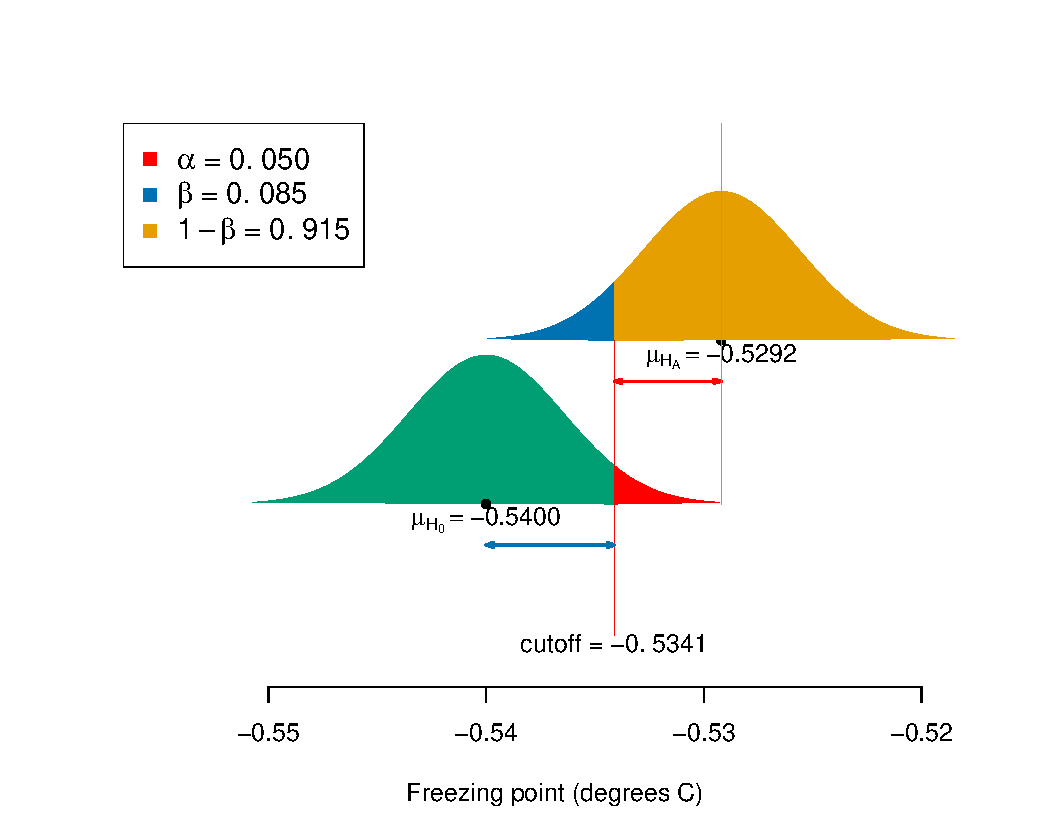
\includegraphics[width=\maxwidth]{figure/unnamed-chunk-8-1} 

}


\end{knitrout}
\end{frame}


\begin{frame}[fragile]{If the supplier added 2\% water to the milk}
\begin{knitrout}\tiny
\definecolor{shadecolor}{rgb}{0.969, 0.969, 0.969}\color{fgcolor}

{\centering \includegraphics[width=\maxwidth]{figure/unnamed-chunk-9-1} 

}


\end{knitrout}
\end{frame}

\begin{frame}[fragile]{If the supplier added 3\% water to the milk}
\begin{knitrout}\tiny
\definecolor{shadecolor}{rgb}{0.969, 0.969, 0.969}\color{fgcolor}

{\centering \includegraphics[width=\maxwidth]{figure/unnamed-chunk-10-1} 

}


\end{knitrout}
\end{frame}



\begin{frame}
	
	\begin{center}
		\includegraphics[scale=0.45]{ProbDetectingWaterInMilk.pdf} 
	\end{center}
	
	\vspace*{-0.18in}
	
	{ \footnotesize
		The probabilities in red were calculated using the formula:
		\texttt{stats::pnorm(cutoff, mean = mu.mixture, sd = SEM, lower.tail=FALSE)}
	}
\end{frame}


\begin{frame}{Statistical Power: the chance of getting caught}
	\begin{itemize}
		\setlength\itemsep{1em}
		\item The calculations shown at the left in the figure on the previous slide are used to set  the cutoff; it is based on the \underline{\textbf{null}} distribution shown at the bottom. \pause  
		\item Clearly the bigger the signal (the `$\Delta$') the more chance the test will `raise the red flag.' It is 92\% when it is a 98:2, and virtually 100\% when it is a 97:3 mix.
	\end{itemize}
	
	
\end{frame}


\section{Assume a 99:1 mix of milk and water. What are the chances of detecting cheating if the buyer uses samples $n$=10, 15 or 20 rather than just 5 measurements?}

\begin{frame}{Power as a function of sample size}
	
	\begin{itemize}
		\setlength\itemsep{1em}
		\item Suppose even a 1\% added water is serious, and worth detecting.
		\item Clearly, from the previous Figure, and again at the bottom row of the following Figure,
		one has only a 45\% chance of detecting it: there is a \textbf{large overlap between the sampling distributions under the null (100\% Milk) and the mixture (99\% milk, 1\% water) scenarios}. \pause 
		
		\item So, to better discriminate, one needs to make a bigger resting effort, and measure more lots,
		i.e., increase the $n$.
	\end{itemize}
\end{frame}


\begin{frame}[fragile]{When the buyer uses samples of size 5}

	
	
\begin{knitrout}\tiny
\definecolor{shadecolor}{rgb}{0.969, 0.969, 0.969}\color{fgcolor}

{\centering 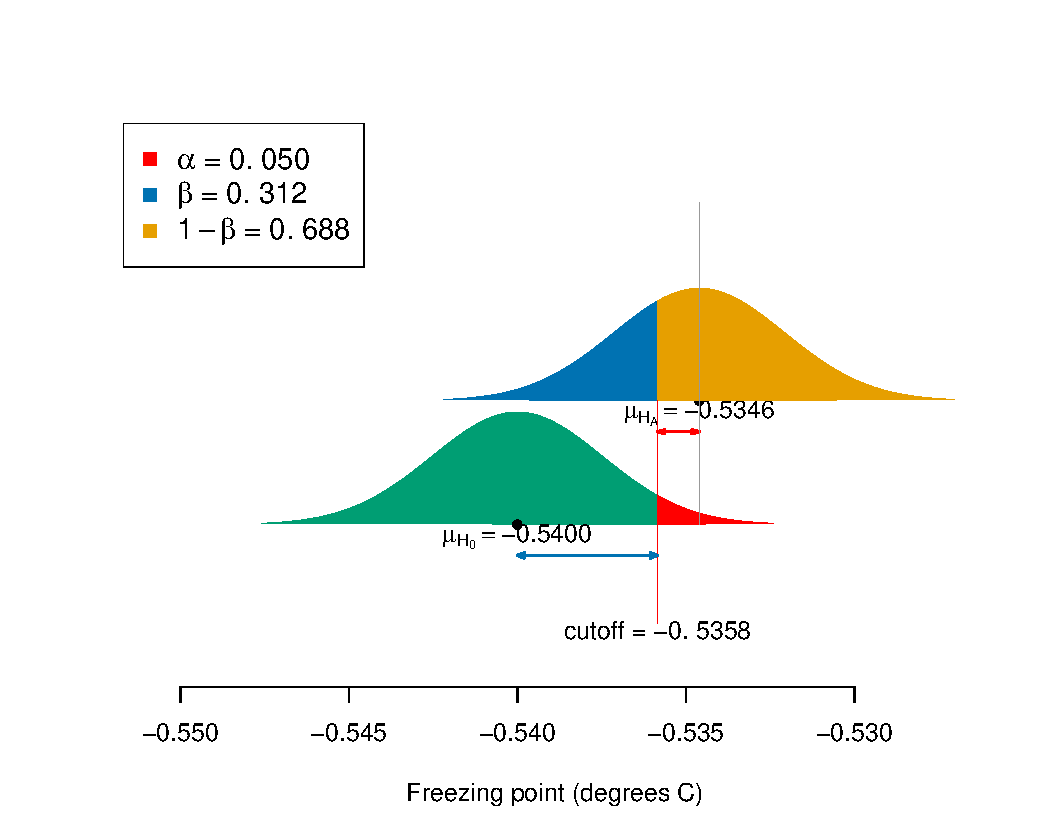
\includegraphics[width=\maxwidth]{figure/unnamed-chunk-12-1} 

}


\end{knitrout}
\end{frame}


\begin{frame}[fragile]{When the buyer uses samples of size 10}
\begin{knitrout}\tiny
\definecolor{shadecolor}{rgb}{0.969, 0.969, 0.969}\color{fgcolor}

{\centering \includegraphics[width=\maxwidth]{figure/unnamed-chunk-13-1} 

}


\end{knitrout}
\end{frame}

\begin{frame}[fragile]{When the buyer uses samples of size 15}
\begin{knitrout}\tiny
\definecolor{shadecolor}{rgb}{0.969, 0.969, 0.969}\color{fgcolor}

{\centering \includegraphics[width=\maxwidth]{figure/unnamed-chunk-14-1} 

}


\end{knitrout}
\end{frame}


\begin{frame}
	\begin{center}
		\includegraphics[scale=0.5]{SampleSize1pctWaterAdded.pdf} 
	\end{center}
\end{frame}


\begin{frame}{Increasing $n$ leads to increased power}
	\begin{itemize}
		\item The larger $n$ narrows and concentrates the sampling distribution. The width is governed by the SD of the sampling distribution of the mean of $n$ measurements, i.e., by the Standard Error of the Mean, or SEM = $\sigma/\sqrt{n}$.\pause 
		
		\item Because the null sampling distribution narrows, the cutoff is brought closer to the null.
		And under the alternative (non-null) scenario, a greater portion of its sampling distribution is to
		the right of (i.e., exceeds) the cutoff. \pause 
		
		\item Indeed, under the alternative (i.e., cheating) scenario the probability of exceeding the threshold  is almost 70\% when $n=10,$ 82\% when $n=15$ and 92\% when n=20. \pause 
		\item 
		You can check these for yourself in \texttt{R} using this expression:\\ \ \\
		{ \footnotesize
			\ \ \ \ \texttt{\textbf{stats::pnorm(cutoff, mean = mu.mixture, sd = sigma/sqrt(n), lower.tail=FALSE)} }  \\ \ \\
		} 
	\end{itemize}
\end{frame}


\section{At what $n$ does the chance of detecting cheating reach 80\%?}

\begin{frame}{What sample size needed?}
	
	\begin{itemize}
		\item We can come up with a closed form formula that (a) allows you to compute the sample size `by hand' and (b) shows you, more explicitly than the diagram or R code can, what drives the $n$.
		
	\end{itemize}
	
\end{frame}

\begin{frame}[fragile]{The balancing formula}
\begin{knitrout}\tiny
\definecolor{shadecolor}{rgb}{0.969, 0.969, 0.969}\color{fgcolor}

{\centering \includegraphics[width=\maxwidth]{figure/unnamed-chunk-15-1} 

}


\end{knitrout}
\end{frame}


\begin{frame}{What sample size needed?}
	
	\begin{itemize}
		\setlength\itemsep{1em}
		\item The `balancing formula', in SEM terms, is simply the $n$ where
		$$ 1.645 \times SEM + 0.84 \times SEM = \Delta.$$
		Replacing each of the  SEMs (assumed equal, because we assumed the variability
		is approx. the same under both scenarios) by $\sigma/\sqrt{n}$,  i.e.,
		
		$$ 1.645 \times \sigma/\sqrt{n} + 0.84 \times \sigma/\sqrt{n} = \Delta.$$
		
		and solving for $n$, one gets
		
		$$  n = (1.645 + 0.84)^2  \times \bigg\{ \frac{\sigma}{\Delta} \bigg\}^2 = 
		(1.645 + 0.84)^2  \times \bigg\{ \frac{Noise}{Signal} \bigg\}^2 .$$
	\end{itemize}
	
\end{frame}


\begin{frame}{What sample size needed?}
	\begin{itemize}
		\setlength\itemsep{1em}
		\item Notice the structure of the formula. The \textit{first} component has to do
		with the operating characteristics or performance of the test, i.e.,
		the type I error probability $\alpha$ and the desired power (the complement of the type II error probability, $\beta$).
		
		\pause 
		
		\item The \textit{second} has to do	with the context in which it is applied, i..e, the size of the noise relative to the  signal. \pause 
		
		\item In our example, where the \underline{Noise-to-Signal Ratio} is $\frac{\sigma = 0.0080}{\Delta = 0.0054}$ = 1.48, so that its square is $1.48^2$ or approx 2.2,	and $(1.645 + 0.84)^2 = 2.485^2$ = approx 6.2,	$$  n = 6.2  \times 2.2  =  13.6, \textrm{approx, or, rounded up,  } n = \textbf{14}. $$
	\end{itemize}
\end{frame}



\begin{frame}[fragile]{Code for null and alternative distribution plots}
\begin{knitrout}\tiny
\definecolor{shadecolor}{rgb}{0.969, 0.969, 0.969}\color{fgcolor}\begin{kframe}
\begin{alltt}
\hlkwd{source}\hlstd{(}\hlstr{"https://raw.githubusercontent.com/sahirbhatnagar/EPIB607/master/inst/code/plot_null_alt.R"}\hlstd{)}

\hlstd{mu0} \hlkwb{<-} \hlopt{-}\hlnum{0.540} \hlcom{# mean under the null}
\hlstd{mha} \hlkwb{<-} \hlnum{0.99}\hlopt{*-}\hlnum{0.540} \hlcom{# mean under the alternative}
\hlstd{s} \hlkwb{<-} \hlnum{0.0080} \hlcom{# sample/population SD}
\hlstd{n} \hlkwb{<-} \hlnum{5} \hlcom{# sample size}
\hlstd{cutoff} \hlkwb{<-} \hlstd{mu0} \hlopt{+} \hlkwd{qnorm}\hlstd{(}\hlnum{0.95}\hlstd{)} \hlopt{*} \hlstd{s} \hlopt{/} \hlkwd{sqrt}\hlstd{(n)}

\hlkwd{power_plot}\hlstd{(}\hlkwc{n} \hlstd{= n,}
\hlkwc{s} \hlstd{= s,}
\hlkwc{mu0} \hlstd{= mu0,}
\hlkwc{mha} \hlstd{= mha,}
\hlkwc{cutoff} \hlstd{= cutoff,}
\hlkwc{alternative} \hlstd{=} \hlstr{"greater"}\hlstd{,}
\hlkwc{xlab} \hlstd{=} \hlstr{"Freezing point (degrees C)"}\hlstd{)}
\end{alltt}
\end{kframe}
\end{knitrout}
\end{frame}





\begin{frame}{Interpreting p-values from statistical tests}
	\begin{itemize}
		\small
		\setlength\itemsep{1em}
		\item In the milk example, an $n=5$ gives an SEM of	$\sigma/\sqrt{5}$ = 0.0080/2236 = 0.0036. So the cutoff for a 1 sided test with $\alpha$ = 0.05 is $1.645 \times 0.0036 = 0.0059$ above -0.5400,
		i.e,. at - 0.5341. 
		\item This is computed under the null (innocence) hypothesis, namely that what we are testing is pure milk, with no added water. \pause 
		\item The 1 sided alternative is that we are testing a `less than 100\%, more than 0\%' mix, where the
		mean is above (to right of) -0.540, i.e., on the (upper) 'added water' side of the null. 
		\item Formally, these two hypotheses are 
		$$\textrm{H}_0: \mu = -0.540; \  H_{alt}: \mu > -0.540.$$
		\pause 
		\item Since the mean of the 5 measurements, namely -0.533$^{\circ}$C, is to the right of (\textbf{exceeds}) this threshold, it would be considered `statistically significant at the 0.05 level.' The actual p-value is \texttt{pnorm(-0.533, mean=-0.54, sd = 0.0036, lower.tail=FALSE)} = \underline{0.026}.
	\end{itemize}
\end{frame}

\begin{frame}{Is this good evidence that the producer is adding water to the milk?}
	\begin{itemize}
		\small
		\setlength\itemsep{1em}
		\pause 
		\item Do  not jump to conclusions and immediately accuse the supplier of cheating
		\pause 
		\item In particular, it would not be appropriate -- or accurate -- to say that you are 1 - 0.026 = 0.974 = 97.4\% certain that the supplier is cheating. 
		\item Remember that a \underline{p-value} is a probability \underline{concerning the data}, \textbf{conditional} on (i.e., computed	under the  assumption that) H$_0$  being (is) true.  In other words, the p-value has to do with P(data $|$ `innocence'), whereas at issue is the reverse,  P(`innocence' $|$ data).
		\pause 
		\item As to this latter probability (of being innocent), there are a lot of other factors to consider first, before accusing the supplier of cheating.
	\end{itemize}
\end{frame}


\begin{frame}{Other factors to consider before accusing the supplier}
	\begin{itemize}
		\small
		\setlength\itemsep{1em}
		\item First, did you (re-)check the calculations?  How recently was the instrument 
		calibrated? etc. \pause 
		\item JH calls these \textbf{Type III errors}: the data were wrong, or the
		instrument was wrong, or the technician mis-calculated something. 
		\item It should remind us that, in the \textit{real} world, there are \textit{many} alternative hypotheses, not just the one.
		\pause 
		\item Second, why did you chose to test \textbf{this} supplier? \pause
		\begin{itemize}
			\item Is it someone that the manager suspected based on previous data, or based on knowing that he is behind in his loan payments to the bank? 
			\item Or maybe the laboratory manager merely asked a technician to start randomly testing, and the first supplier (blindly) chosen was the manager's brother-in-law?
		\end{itemize}
	\end{itemize}
\end{frame}



\begin{frame}{Are all $p$-values created equal?}
	\begin{itemize}
		\small
		\setlength\itemsep{1em}
		\item So, you can see that, just as in medical tests, there are\textbf{ many other pieces of evidence} or information, or circumstances, besides the $p$-value, that bear on the probability of innocence or guilt.
		\item This is very nicely brought out in the article `Are all p-values created equal?' which you can
		here: { \footnotesize \url{http://www.biostat.mcgill.ca/hanley/BionanoWorkshop/AreAllSigPValuesCreatedEqual.pdf}}
		
		\item Sadly, the mixing up of P(data $|$ hypothesis) and P(data $|$ data) -- often referred to as
		`The Prosecutor's Fallacy' -- is  common, and can lead to serious harm. 
	\end{itemize}
\end{frame}


\begin{frame}{When does the $p$-value work well?}
	\begin{itemize}
		\small
		\setlength\itemsep{1em}
		\item The use of $p$-values works well in \underline{Quality Control}, where the aim is to detect
		(the \underline{few})  deviations ('\underline{bad}' ones)  from the desired specifications, to stop and fix	the offending machine, or to flag defective batches. \pause 
		\item It is not clear that it is equally effective at identifying the (\underline{few}) truly active (`{good}) compounds	via the mass testing of lots of compounds, most of which are expected to be inactive -- and then investing all one's effort in these few `good' ones at the next stage of development.
	\end{itemize}
\end{frame}


\section{Another example on power: Lake Wobegon}

\begin{frame}[fragile]{Power: Lake Wobegon}
	\small
	\begin{itemize}
		\item It is claimed that the children of Lake Wobegon are above
		average. Take a simple random sample of 9 children from Lake
		Wobegon, and measure their IQ to obtain a sample mean of 112.8. 
		\item IQ scores are scaled to be Normally distributed with mean 100 and
		standard deviation 15. 
%		\item Does this sample provide evidence to reject the null hypothesis of no difference between children of Lake Wobegon and the general population? \pause 
		\item[]\item[1.] \textcolor{blue}{Null and alternative hypotheses:} The claim made is
		that the population of children Lake Wobegon have higher than
		average intellidence. Thus the null hypothesis is that the
		population has average intelligence, or a score of 100. Therefore
		$H_0: \mu=100$, and the (one-sided) alternative is $H_A: \mu >
		100$.
	\end{itemize}
\end{frame}


\begin{frame}[fragile]{Lower limit of 95\% CI}
	\small
	\begin{enumerate}
		\item \underline{Hypotheses.} $H_0: \mu = 100$, $H_A: \mu > 100$.
		\item \underline{Calculate 95\% CI.}
\begin{knitrout}\tiny
\definecolor{shadecolor}{rgb}{0.969, 0.969, 0.969}\color{fgcolor}\begin{kframe}
\begin{alltt}
\hlstd{mosaic}\hlopt{::}\hlkwd{xqnorm}\hlstd{(}\hlkwc{p} \hlstd{=} \hlkwd{c}\hlstd{(}\hlnum{0.05}\hlstd{,}\hlnum{1}\hlstd{),} \hlnum{112.8}\hlstd{,} \hlnum{15}\hlopt{/}\hlkwd{sqrt}\hlstd{(}\hlnum{9}\hlstd{))}
\end{alltt}
\end{kframe}

{\centering \includegraphics[width=\maxwidth]{figure/unnamed-chunk-17-1} 

}


\begin{kframe}\begin{verbatim}
## [1] 104.5757      Inf
\end{verbatim}
\end{kframe}
\end{knitrout}
		\pause 
		\item \underline{Statement.} The lower limit of the CI excludes $\mu_0=100$, and so \underline{there is evidence to suggest} that the children at Lake Wobegon are brighter than other children at the $\alpha=0.05$ level.
	\end{enumerate}
	
\end{frame}

\frame{\frametitle{Power} Steps to finding power:
	\begin{enumerate}
		\item State null hypothesis, $H_0$, and state a specific alternative, $H_A$, as the minimum (clinical/substantive) departure from the null hypothesis that would
		be of interest. \pause
		\item Find the values of $\overline{y}$ that lead to rejection of
		$H_0$. \pause
		\item Calculate the probability of observing the values found in
		(2) when the alternative is true.
	\end{enumerate}
} \frame{\frametitle{Power} Example: Lake Wobegon\\
	Suppose you hope to use a \textbf{one-sided} test to show that the children from Lake
	Wobegon are at least 10 points higher than average on the IQ test. What power do you have
	to detect this with the sample of 9 children if using a 0.05-level test? \\ \ \\ \pause
	\begin{enumerate}
		\item \underline{Hypotheses.} $H_0: \mu = 100$, $H_A: \mu > 110$. \pause
		\item[] \item \underline{Find values of the sample mean that reject the
			null.}\\ \ \\ The test will reject $H_0$ at the 0.05 level whenever
		\[z = \frac{\overline{y}-\mu_0}{\sigma/\sqrt{n}} =
		\frac{\overline{y}-100}{15/\sqrt{9}} \ge 1.645.\] Now we must
		translate this back to values of $\overline{y}$...
	\end{enumerate}
} \frame{\frametitle{Power} Example: Lake Wobegon\\
	\begin{enumerate}
		\item[2.] \underline{Values of the sample mean that reject $H_0$
			(con't)}\\ \ \\
		The test will reject $H_0$ at the 0.05 level whenever \[
		\frac{\overline{y}-100}{15/\sqrt{9}} \ge 1.645,\] which means we
		reject $H_0$ whenever \[ \overline{y} \ge 1.645\times 15/\sqrt{9}+100 = 108.2\]
		If $H_0$ is true, the probability of seeing an IQ score as big as
		108.2 or bigger is 5\%.
	\end{enumerate}
} \frame{\frametitle{Power} Example: Lake Wobegon\\
	\begin{enumerate}
		\item[3.] \underline{Find the probability of rejecting $H_0$ if
			$\mu=\mu_A=110$.}\\ \ \\
		$P(\overline{y} > 108.2|\mu=\mu_A=110) $
		\begin{eqnarray*} \qquad \qquad & = &
			P\left(\left.\frac{\overline{y}-\mu_A}{\sigma/\sqrt{n}}
			> \frac{108.2-110}{15/\sqrt{9}}\right|\mu=\mu_A=110\right)\\
			& = & P\left(z > -0.36\right)\\
			& = & 0.64\\
		\end{eqnarray*}
		So there is approximately a 2/3 chance of detecting a difference of
		10 points on the IQ scale at the 0.05 level of significance with a
		sample size of 9.
	\end{enumerate}
} 


\begin{frame}[fragile]{Null and alternative distribution plots}
\begin{knitrout}\tiny
\definecolor{shadecolor}{rgb}{0.969, 0.969, 0.969}\color{fgcolor}\begin{kframe}
\begin{alltt}
\hlkwd{source}\hlstd{(}\hlstr{"https://raw.githubusercontent.com/sahirbhatnagar/EPIB607/master/inst/code/plot_null_alt.R"}\hlstd{)}
\hlkwd{power_plot}\hlstd{(}\hlkwc{n} \hlstd{=} \hlnum{9}\hlstd{,} \hlkwc{s} \hlstd{=} \hlnum{15}\hlstd{,} \hlkwc{mu0} \hlstd{=} \hlnum{100}\hlstd{,} \hlkwc{mha} \hlstd{=} \hlnum{110}\hlstd{,}
\hlkwc{cutoff} \hlstd{=} \hlnum{100} \hlopt{+} \hlkwd{qnorm}\hlstd{(}\hlnum{0.95}\hlstd{)} \hlopt{*} \hlnum{15} \hlopt{/} \hlkwd{sqrt}\hlstd{(}\hlnum{9}\hlstd{),}
\hlkwc{alternative} \hlstd{=} \hlstr{"greater"}\hlstd{,} \hlkwc{xlab} \hlstd{=} \hlstr{"Average IQ Score"}\hlstd{)}
\end{alltt}
\end{kframe}

{\centering \includegraphics[width=\maxwidth]{figure/unnamed-chunk-18-1} 

}


\end{knitrout}
\end{frame}



\frame{\frametitle{Power} Example: Lake Wobegon\\ \ \\
	If you hoped to use a \underline{two-sided test} to show that the children from Lake Wobegon are at
	least 10 points higher than average on the IQ test, what power do you have with the
	sample size of 9 and a 0.05-level test? \pause
	\begin{enumerate}
		\item \underline{Hypotheses.} $H_0: \mu = 100$, $H_A: \mu = 110$.\pause 
		\item[] \item \underline{Find values of the sample mean that reject the
			null.}\\ \ \\ The test will reject $H_0$ at the 0.05 level whenever
		\[z = \frac{\overline{y}-\mu_0}{\sigma/\sqrt{n}} =
		\frac{\overline{y}-100}{15/\sqrt{9}} \ge \textcolor{red}{1.96}
		\qquad \hbox{\textbf{\textcolor{blue}{OR when}}}\]
		\[z = \frac{\overline{y}-\mu_0}{\sigma/\sqrt{n}} =
		\frac{\overline{y}-100}{15/\sqrt{9}} \le \textcolor{red}{-1.96}\]
		since we are performing a two-sided test.
	\end{enumerate}
} \frame{\frametitle{Power} Thus we reject $H_0$ if $\overline{y}
	\ge 1.96\times5+100 = 109.8$ \textbf{OR} if $\overline{y} \le
	-1.96\times5+100 = 90.2$
	\begin{enumerate}
		\item[3.] \underline{Find the probability of rejecting $H_0$ if
			$\mu=\mu_A=110$.}\\ \ \\
		$P(\overline{y} > 109.8 \hbox{\textbf{ OR }} \overline{y} <
		90.2|\mu=\mu_A=110) $
		\begin{eqnarray*} \qquad & = & P(\overline{y} >
			109.8|\mu_A=110) + P(\overline{y} < 90.2|\mu_A=110)\\
			& = & P\left(\left.\frac{\overline{y}-\mu_A}{\sigma/\sqrt{n}}
			> \frac{109.8-110}{15/\sqrt{9}}\right|\mu_A=110\right)\\
			&  & \quad + P\left(\left.\frac{\overline{y}-\mu_A}{\sigma/\sqrt{n}}
			< \frac{90.2-110}{15/\sqrt{9}}\right|\mu_A=110\right)\\
			& = & P\left(z > -0.04\right) + P\left(z < -3.96\right)\\
			& = & 0.52 + 3.7\times10^{-5} \approx 0.52\\
		\end{eqnarray*}
		There is about a 1/2 chance of detecting a difference of 10 pts on
		the IQ scale at the 0.05 level of significance with $n=9$ using a
		two-sided alternative hypothesis.
	\end{enumerate}
} \frame{\frametitle{Power} 
	\small 
	
	\begin{itemize}
		\item Steps 1 and 2 used to find the power of a one-sided test to detect a difference of $x$ points above (or below) the population mean are similar to the steps for finding the power of a two-sided test to detect a difference of $x$ points on either side of the population mean. 
		\item However for a two-sided test, there will be two sets of values of $\overline{y}$
		that lead us to reject $H_0$ (also, $z_\alpha$ for one-sided and
		$z_{\alpha/2}$ for two-sided).  %\pause
		
		\item \textbf{However}, there is one critical difference in the third step: we need to
		calculate the probability of seeing $\overline{y}$ in either of the two tails (rejection
		regions) of the null distribution under the assumption that the true distribution has
		mean $\mu_A$. So there will be two probabilities to calculate in the third step. 
		\pause
		
		\item Note: If we felt that the minimum significant departure from $\mu_0$
		was different above and below (e.g., we are interested in increases
		of blood pressure of at least 3.5mmHg and decreases of blood
		pressure of at least 2mmHg), we perform the calculations as though
		we were interested in the minimum of the two values (Why?).
	\end{itemize}
} 

\frame{\frametitle{Power} Exercises: Lake Wobegon\\ \ \\
	Find the power of the following tests, assuming two-sided
	alternative hypotheses:
	\begin{enumerate}
		\item A 0.05-level test to detect a difference of 15 points on the
		IQ scale using the 9 children.
		\item A 0.05-level test to detect a difference of 5 points on the
		IQ scale using the 9 children.
		\item A 0.05-level test to detect a difference of 10 points on the
		IQ scale using 25 children.
		\item A 0.01-level test to detect a difference of 10 points on the
		IQ scale using the 9 children.
\end{enumerate} }


\begin{frame}[fragile]{Session Info}
	\tiny
	
\begin{knitrout}\tiny
\definecolor{shadecolor}{rgb}{0.969, 0.969, 0.969}\color{fgcolor}\begin{kframe}
\begin{verbatim}
R version 4.1.1 (2021-08-10)
Platform: x86_64-pc-linux-gnu (64-bit)
Running under: Pop!_OS 21.04

Matrix products: default
BLAS:   /usr/lib/x86_64-linux-gnu/openblas-pthread/libblas.so.3
LAPACK: /usr/lib/x86_64-linux-gnu/openblas-pthread/libopenblasp-r0.3.13.so

attached base packages:
[1] tools     stats     graphics  grDevices utils     datasets  methods  
[8] base     

other attached packages:
 [1] DT_0.16           mosaic_1.7.0      Matrix_1.3-2      mosaicData_0.20.1
 [5] ggformula_0.9.4   ggstance_0.3.4    lattice_0.20-41   kableExtra_1.2.1 
 [9] socviz_1.2        gapminder_0.3.0   here_0.1          NCStats_0.4.7    
[13] FSA_0.8.30        forcats_0.5.1     stringr_1.4.0     dplyr_1.0.7      
[17] purrr_0.3.4       readr_1.4.0       tidyr_1.1.3       tibble_3.1.5     
[21] ggplot2_3.3.5     tidyverse_1.3.0   knitr_1.36       

loaded via a namespace (and not attached):
 [1] fs_1.5.0           lubridate_1.7.9    webshot_0.5.2      httr_1.4.2        
 [5] rprojroot_2.0.2    latex2exp_0.4.0    backports_1.2.1    utf8_1.2.2        
 [9] R6_2.5.1           DBI_1.1.1          colorspace_2.0-2   withr_2.4.2       
[13] tidyselect_1.1.1   gridExtra_2.3      leaflet_2.0.3      curl_4.3.2        
[17] compiler_4.1.1     cli_3.0.1          rvest_1.0.0        pacman_0.5.1      
[21] xml2_1.3.2         ggdendro_0.1.22    labeling_0.4.2     mosaicCore_0.8.0  
[25] scales_1.1.1       digest_0.6.28      foreign_0.8-81     rmarkdown_2.11.3  
[29] rio_0.5.16         pkgconfig_2.0.3    htmltools_0.5.2    highr_0.9         
[33] dbplyr_1.4.4       fastmap_1.1.0      htmlwidgets_1.5.3  rlang_0.4.11      
[37] readxl_1.3.1       rstudioapi_0.13    farver_2.1.0       generics_0.1.0    
[41] jsonlite_1.7.2     crosstalk_1.1.1    zip_2.2.0          car_3.0-9         
[45] magrittr_2.0.1     Rcpp_1.0.7         munsell_0.5.0      fansi_0.5.0       
[49] abind_1.4-5        lifecycle_1.0.1    stringi_1.7.5      carData_3.0-4     
[53] MASS_7.3-53.1      plyr_1.8.6         grid_4.1.1         blob_1.2.1        
[57] ggrepel_0.8.2      crayon_1.4.1       cowplot_1.1.0      haven_2.3.1       
[61] splines_4.1.1      hms_1.1.1          pillar_1.6.3       reprex_0.3.0      
[65] glue_1.4.2         evaluate_0.14      data.table_1.14.2  modelr_0.1.8      
[69] vctrs_0.3.8        tweenr_1.0.1       cellranger_1.1.0   gtable_0.3.0      
[73] polyclip_1.10-0    assertthat_0.2.1   TeachingDemos_2.12 xfun_0.26         
[77] ggforce_0.3.2      openxlsx_4.1.5     broom_0.7.2        viridisLite_0.4.0 
[81] ellipsis_0.3.2    
\end{verbatim}
\end{kframe}
\end{knitrout}
	
\end{frame}

\end{document}


\end{document}
